\documentclass[14pt,red]{beamer}
\usepackage{beamerthemesplit}
\usetheme{Warsaw}
\usepackage{amsmath, amssymb,graphicx, natbib, setspace, times}
\definecolor{DarkRed2}{rgb}{0.6,0.00,0.08}
\newcommand{\indep}{{\;\bot\!\!\!\!\!\!\bot\;}}
\beamertemplateballitem

\title[\texttt{eiPack}: R $\times$ C Ecological Inference and Data
Management]{{\small \texttt{eiPack}: Tools for R $\times$ C Ecological
Inference and Higher-Dimension Data Management}}
\author[Olivia Lau, Ryan T. Moore, Michael Kellermann]{{\footnotesize Olivia Lau \and Ryan T. Moore \and Michael Kellermann}}
\institute{Department of Government \\ Institute for Quantitative Social
Science\\Harvard University}

\date{{\footnotesize Vienna, Austria\\ \vspace{-6pt}16 June 2006}}
\logo{\includegraphics[height=0.5cm]{useR-large.png}}

\begin{document}
\frame{\titlepage}

\frame{
\frametitle{What is ecological inference ({\sc ei})?}

\begin{itemize}
\item Goal:  infer individual level behavior from aggregate data
\item Unit of analysis: contingency table with observed marginals
{\small
\begin{center}
\begin{tabular}{l|ccc|c}
	& $col_1$ & $col_2$ & $col_3$ & \\
\hline
$row_1\quad$	& \color{DarkRed2}{$\quad N_{11i}\quad$} &
\color{DarkRed2}{$\quad N_{12i}\quad$} &
\color{DarkRed2}{$\quad N_{13i}\quad$} & $\quad N_{1\cdot i}$ \\
$row_2\quad$ 	& \color{DarkRed2}{$N_{21i}$} & \color{DarkRed2}{$N_{22i}$} &
\color{DarkRed2}{$N_{23i}$} & $\quad N_{2\cdot i}$ \\ 
$row_3\quad$	& \color{DarkRed2}{$N_{31i}$} & \color{DarkRed2}{$N_{32i}$} &
\color{DarkRed2}{$N_{33i}$} & $\quad N_{3\cdot i}$ \\ 
\hline
	& $N_{\cdot 1i}$ & $N_{\cdot 2i}$ & $N_{\cdot 3i}$ & $\quad N_i$
\end{tabular} 
\end{center}
} \pause
\item \texttt{eiPack} methods estimate unobserved internal cells (or functions
thereof) 
\end{itemize} 
}

\frame{
\frametitle{\texttt{eiPack}}
\begin{itemize}
\item Other packages focus on $2\times2$ inference (e.g.,
\texttt{eco}, \texttt{MCMCpack})
\item \texttt{eiPack}: $R \times C$ inference \pause
\item \texttt{eiPack} methods:
	\begin{itemize}
\item Method of bounds
\item Ecological regression 
\item Multinomial-Dirichlet model
	\end{itemize} \pause
\item \texttt{eiPack} data: \texttt{senc}
	\begin{itemize}
	\item Individual level party affiliation 
	\item Black, White, and Native American voters 
	\item 8 counties (212 precincts) in SE North Carolina 
	\item Cell counts known
	\end{itemize} 
\end{itemize}
}

\frame{
\frametitle{\texttt{eiPack}}
\noindent{The models implemented in \texttt{eiPack} share:} \pause
\begin{itemize}
\item A common input syntax of the form: \\
{\footnotesize \texttt{cbind(col1, ..., colC) $\sim$ cbind(row1,
...,rowR)}} 
\item Functions to calculate proportions of some subset of columns 
% -- e.g. 2-party share of affiliation: {\footnotesize \texttt{lambda.reg},
%\texttt{lambda.MD}, \ldots} 
\item Appropriate \texttt{print}, \texttt{summary}, and \texttt{plot} functions
\end{itemize}
}

\frame{
\frametitle{Method of bounds}
\begin{itemize}
\item Quantity of interest: proportion of row members in each column
for each unit 
\item Observed row and column marginals determine upper and lower
bounds \pause
\item Row thresholds implemented for \textit{extreme case analysis} \pause
%\item {\small \begin{displaymath}
%\frac{\max(0, N_j - \sum_{k \neq k'} N_k)}{\max(0, N_j - \sum_{k \neq
%k'} N_k) + \min(N_j, \sum_{k \in k''} N_k)} < \frac{N_{jk'}}{N_{jk'} +
%\sum_{k \in k''} N_{jk}} < \frac{\min(N_j, N_{k'})}{\min(N_j, N_{k'}) + \max(0, N_j - N_{k'} - \sum_{k \in \tilde{k}} N_k)}
%\end{displaymath}}
\item Output:\\
\texttt{ \$white.dem\\
\begin{tabular}{lrr}
 &        lower &    upper \\
18 & 0.519 & 0.559 \\
25 & 0.450 & 0.469 \\
28 & 0.392 & 0.487
\end{tabular}
}
\end{itemize}
}

\frame{
\frametitle{Method of bounds}
\begin{center}
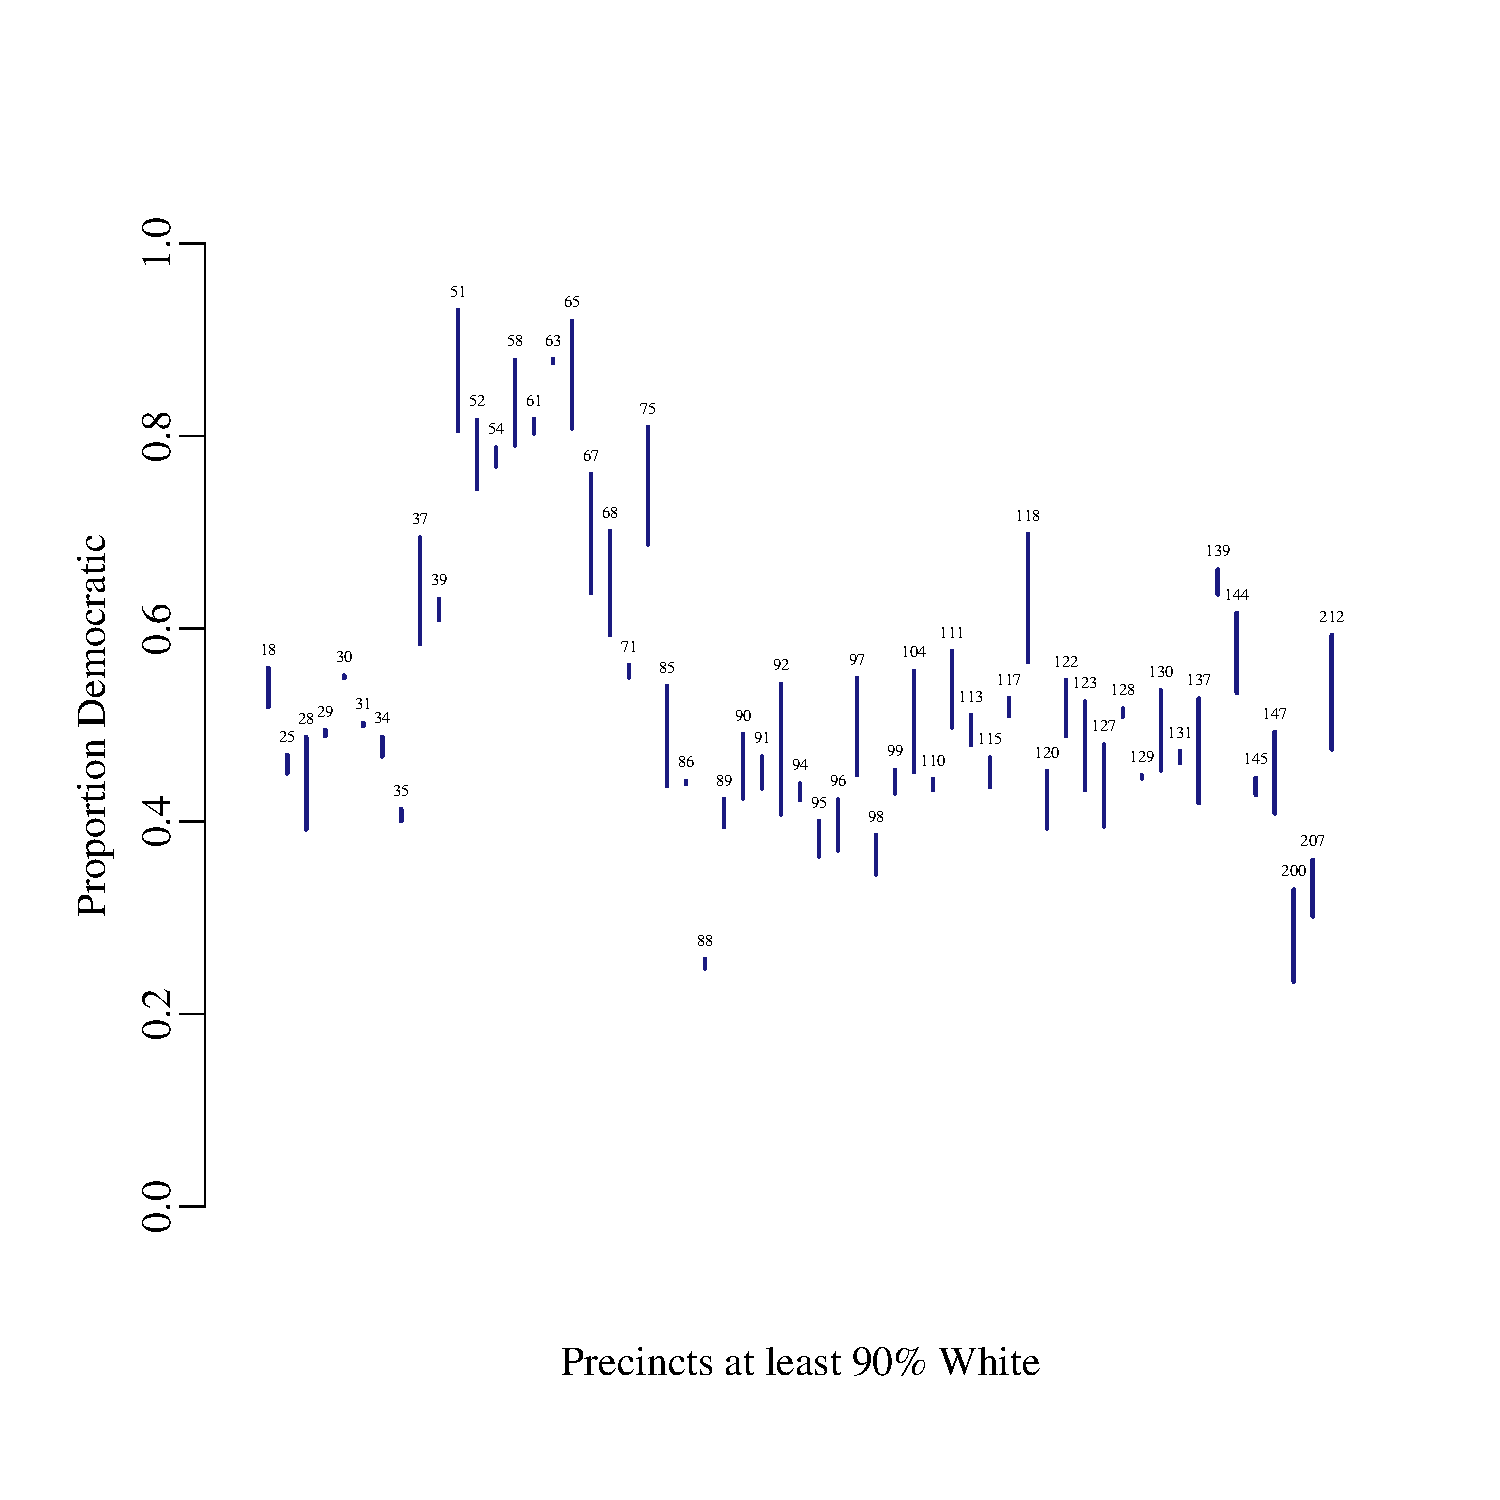
\includegraphics[width=3.2in]{whitenodots.pdf}
\end{center}
}

\frame{
\frametitle{Method of bounds}
\begin{center}
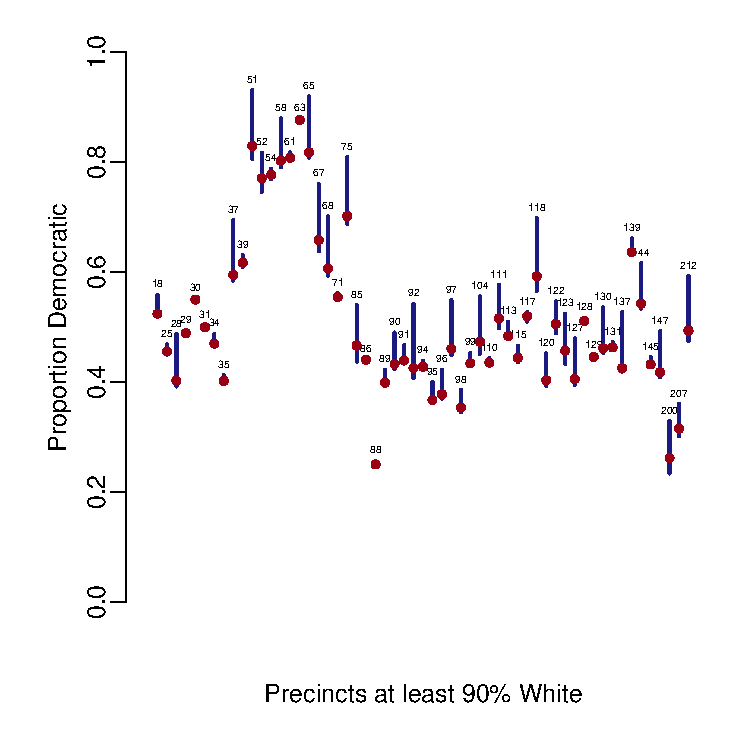
\includegraphics[height=3.2in]{white.pdf}
\end{center}
}

\frame{
\frametitle{Ecological regression}
\begin{itemize}
\item Express data as proportions of row totals
\item Regress each column on all row proportions ($C$ regressions) 
\item Coefficients estimate cell proportions \pause
\item \texttt{eiPack}: freq. and Bayesian regression \pause
%\item Identities: 
%\begin{eqnarray*}
%T_{ci} & = & \sum_{r=1}^R \beta_{rci} X_{ri} \\
%\sum_{c=1}^{C} \beta_{rci}  & = & 1    
%\end{eqnarray*}
%\item Define the population cell fractions $\beta_{rc}$ such that
%$\sum_{c=1}^C \beta_{rc}  =  1$ for every $r$.  Assuming that
%$\beta_{rci} = \beta_{rc}$ for all $i$, estimating the regression
%equations $T_{ci} = \beta_{rc} X_{ri} + \epsilon_{ci}$ recovers the
%population parameters $\beta_{rc}$ when the standard linear regression
%assumptions apply, including $E[\epsilon_{ci}] = 0$ and $Var[\epsilon_{ci}] = \sigma_c^2$ for all $i$.
%\item \begin{verbatim}
%ei.reg(cbind(dem, rep, non) ~ cbind(black, white, natam), 
%   data = senc)
%\end{verbatim}
%\item \texttt{summary} output like \texttt{lm}
\item \texttt{lambda} functions calculate shares of a subset of
columns -- e.g. ``among Blacks, Dem. share of 2-party registration''
%\item Here's
%\begin{verbatim} 
%lambda.reg(out.reg, columns = c("dem", "rep")) 
%\end{verbatim}
%\item \texttt{density.plot} provides a graphical summary of \texttt{lambda} output:
\end{itemize}
}

\frame{
\frametitle{Ecological regression}
\begin{center}
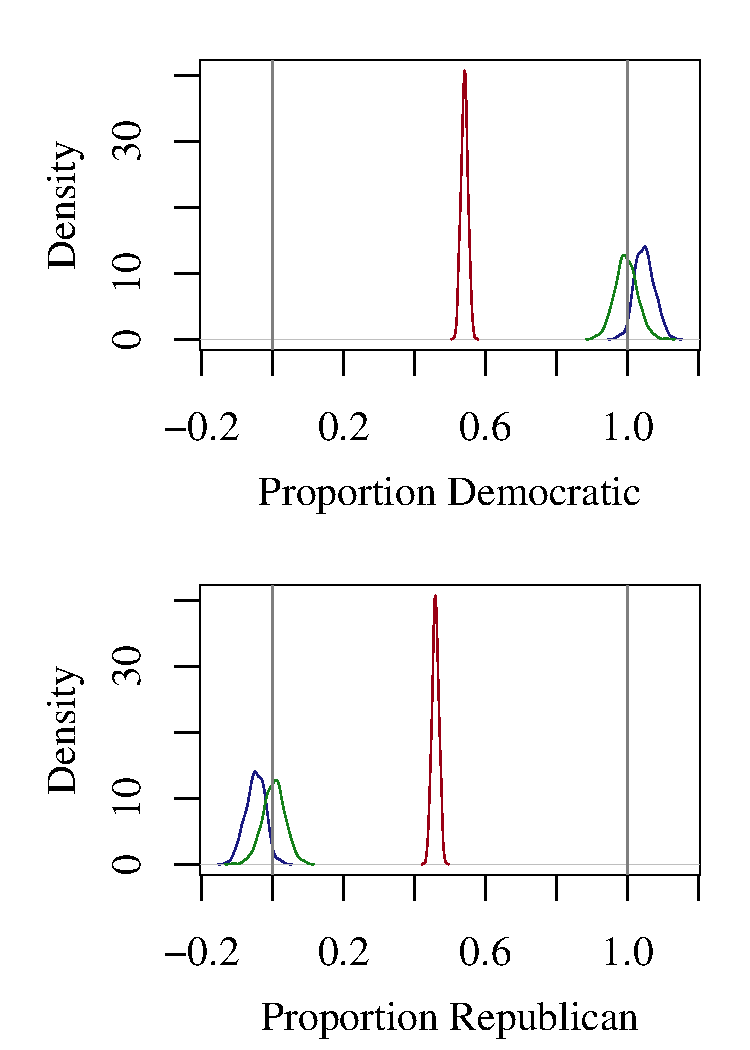
\includegraphics[height=3in]{eiBayesReg.pdf}
\end{center}
}

\frame{
\frametitle{Multinomial-Dirichlet ({\sc md}) model}

\begin{itemize}
\item Express data as counts
\item Fit hierarchical Bayesian model
	\begin{itemize}
	\item Level 1: column marginals $\sim Multinomial$, $\indep$
across units  
	\item Level 2: rows of cell fractions $\sim Dirichlet$,
$\indep$ across rows and units
	\item Level 3: Dirichlet parameters $\sim Gamma$, i.i.d.
	\end{itemize} \pause
%\item Without covariate
%\begin{eqnarray*}
%(N_{\cdot 1i}, \dots, N_{\cdot Ci}) &\stackrel{\indep}{\sim}& {\rm Multinomial}(N_i,
%\sum_{r=1}^R \beta_{r1i}X_{ri}, \dots, \sum_{r=1}^R \beta_{rCi}X_{ri}) \\
%(\beta_{r1i}, \dots, \beta_{rCi}) &\stackrel{\indep}{\sim}& {\rm
%Dirichlet}(\alpha_{r1}, \dots, \alpha_{rC}) \; \forall \; r = 1,\dots, R \\
%\alpha_{rc} &\stackrel{\rm i.i.d.}{\sim}& {\rm
%Gamma}(\lambda_1,\lambda_2) 
%\end{eqnarray*}
%\item With a covariate $Z_i$
%\begin{eqnarray*}
%(N_{\cdot 1i}, \dots, N_{\cdot Ci}) &\stackrel{\indep}{\sim}& {\rm Multinomial}(N_i,
%\sum_{r=1}^R \beta_{r1i}X_{ri}, \dots, \sum_{r=1}^R \beta_{rCi}X_{ri}) \\
%(\beta_{r1i}, \dots, \beta_{rCi}) &\stackrel{\indep}{\sim}& {\rm
%Dirichlet}\left(d_r\exp(\gamma_{rc} + \delta_{rc}Z_i), \dots, \right. \\
%& & \quad\quad \left. d_r\exp(\gamma_{r(C-1)} +
%\delta_{r(C-1)}Z_i), d_r \right) \\
%d_r &\stackrel{\rm i.i.d.}{\sim}& {\rm Gamma}(\lambda_1, \lambda_2)  
%\end{eqnarray*}
%\begin{itemize}
%\item Priors on each $\gamma_{rc}$ and $\delta_{rc}$ are improper
%\item Parameterization of prior on each $(\beta_{r1i}, \dots,
%\beta{rCi})$ is linear with respect to the covariate $Z_i$ in the
%log-odds ratio of the expected fractions
%\begin{displaymath}
%\log\left( \frac{E(\beta_{rci})}{E(\beta_{rCi})} \right) = \gamma_{rc}
%+ \delta_{rc} Z_i
%\end{displaymath}
%\end{itemize}
%\item \begin{verbatim}
%ei.MD.bayes(cbind(dem, rep, non) ~ cbind(black, white, 
%   natam), covariate = NULL, data = senc, lambda1 = 4, 
%   lambda2 = 2,  tune.list = tune.nocov, start.list = NULL, 
%   sample = 1000, thin = 5000, burnin = 1000000, 
%   ret.beta = 'r', ret.mcmc = TRUE, usrfun = NULL)
%\end{verbatim}
\item \texttt{lambda} and \texttt{density.plot} functions
\end{itemize}
}

\frame{
\frametitle{Multinomial-Dirichlet ({\sc md}) model}
%\begin{verbatim}
%cover.plot(out.nocov, row = "white", column = "dem")
%\end{verbatim}
\begin{center}
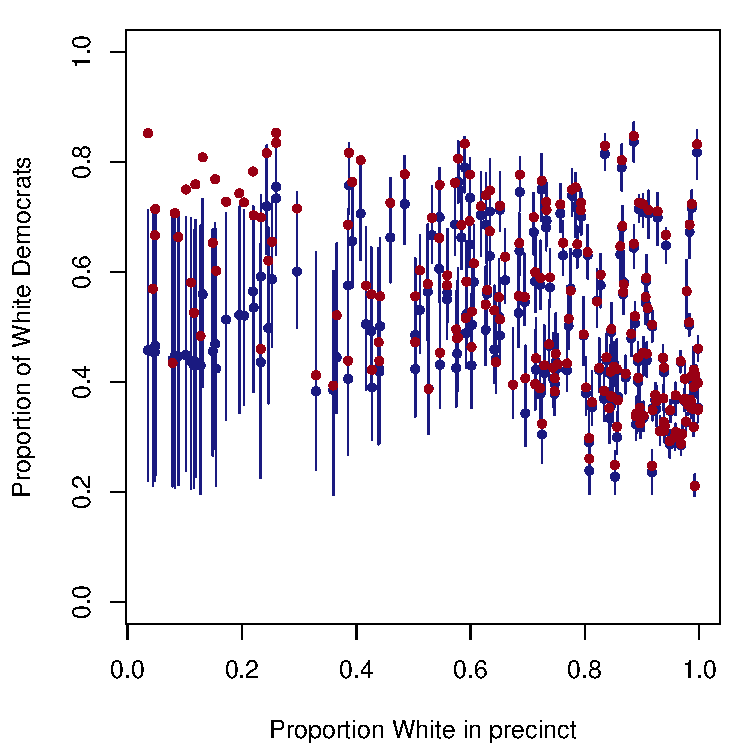
\includegraphics[width=3in]{coversmall.pdf}
\end{center}
}


\frame{
\frametitle{Data Management}
\begin{itemize}
\item Reasonable-sized problems produce unreasonable amounts of data \pause
\item E.g., a model for voting in Ohio includes
	\begin{itemize}
	\item 11000 precincts
	\item 3 racial groups
	\item 4 party options
	\end{itemize} \pause
\item 1000 iterations yields about $1.3 \times 10^8$ parameter draws
\item Draws occupy $\approx$ 1{\sc gb} of {\sc ram}; probably not
enough iterations  \pause
\item \texttt{eiPack} allows users to write chains to disk, or discard
chains not of interest
\end{itemize}
}

\frame{
\begin{center} Visit our poster for more! \end{center}
}

\end{document}
